\documentclass[tikz,border=10pt]{standalone}
\usepackage{tikz}
\usetikzlibrary{shapes,arrows,positioning,fit,backgrounds}

\begin{document}
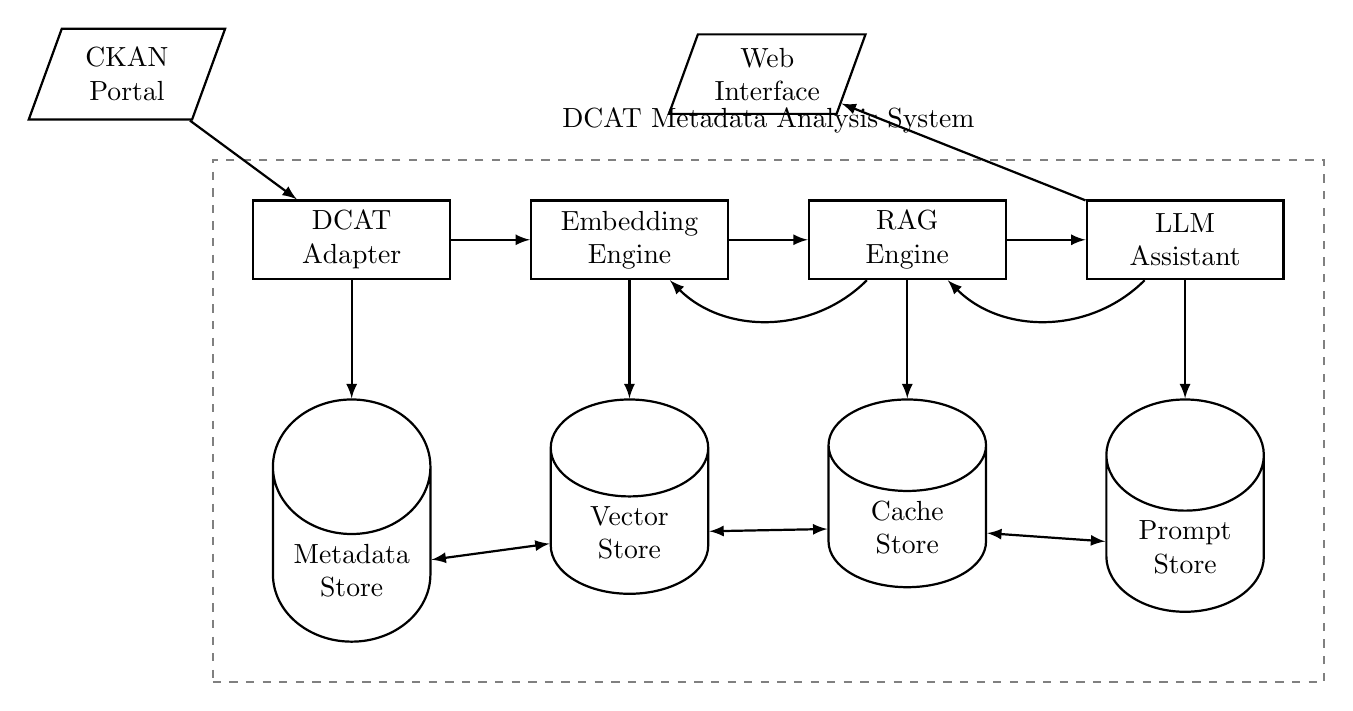
\begin{tikzpicture}[
    node distance=1.5cm,
    box/.style={
        rectangle,
        draw=black,
        thick,
        minimum height=1cm,
        minimum width=2.5cm,
        align=center
    },
    interface/.style={
        draw=black,
        thick,
        trapezium,
        trapezium left angle=70,
        trapezium right angle=110,
        minimum height=1cm,
        minimum width=2.5cm,
        align=center
    },
    database/.style={
        cylinder,
        draw=black,
        thick,
        shape border rotate=90,
        minimum height=1cm,
        minimum width=2cm,
        align=center
    },
    arrow/.style={
        ->,
        >=latex,
        thick
    }
]

% External Systems
\node[interface] (ckan) {CKAN\\Portal};
\node[interface, right=6cm of ckan] (user) {Web\\Interface};

% Core Components
\node[box, below right=1cm and 1cm of ckan] (adapter) {DCAT\\Adapter};
\node[box, right=1cm of adapter] (embedding) {Embedding\\Engine};
\node[box, right=1cm of embedding] (rag) {RAG\\Engine};
\node[box, right=1cm of rag] (llm) {LLM\\Assistant};

% Databases
\node[database, below=1.5cm of adapter] (metadata_db) {Metadata\\Store};
\node[database, below=1.5cm of embedding] (vector_db) {Vector\\Store};
\node[database, below=1.5cm of rag] (cache_db) {Cache\\Store};
\node[database, below=1.5cm of llm] (prompt_db) {Prompt\\Store};

% Background System Boundary
\begin{scope}[on background layer]
\node[rectangle, draw=gray, dashed, thick, fit=(adapter) (embedding) (rag) (llm) (metadata_db) (vector_db) (cache_db) (prompt_db), inner sep=0.5cm] (system) {};
\node[above=0.2cm of system] {DCAT Metadata Analysis System};
\end{scope}

% Connections
\draw[arrow] (ckan) -- (adapter);
\draw[arrow] (adapter) -- (embedding);
\draw[arrow] (embedding) -- (rag);
\draw[arrow] (rag) -- (llm);
\draw[arrow] (llm) -- (user);

% Database connections
\draw[arrow] (adapter) -- (metadata_db);
\draw[arrow] (embedding) -- (vector_db);
\draw[arrow] (rag) -- (cache_db);
\draw[arrow] (llm) -- (prompt_db);

% Bidirectional connections
\draw[arrow, <->] (metadata_db) -- (vector_db);
\draw[arrow, <->] (vector_db) -- (cache_db);
\draw[arrow, <->] (cache_db) -- (prompt_db);

% Feedback loops
\draw[arrow, bend left=45] (llm) to (rag);
\draw[arrow, bend left=45] (rag) to (embedding);

\end{tikzpicture}
\end{document} 